\chapter{Automatische Segmentierung mittels 3D Slicer}
\label{sec:3d_slicer} 3D Slicer ist eine Open-Source-Plattform, die speziell für
die Verarbeitung von Bilddaten im medizinischen Kontext eingesetzt wird. Dabei wird
sie von einer aktiven Community regelmäßig gewartet und weiterentwickelt \citep[vgl.][]{slicer2024},
\citep[vgl.][S.~1325]{fedorov2012slicer}. Für Slicer gibt es offiziell keine Nutzungsbeschränkung.
Jedoch sei auch gesagt, dass 3D Slicer nicht für die klinische Nutzung zugelassen
ist. \citet[S.~1331]{fedorov2012slicer} machen deutlich, dass 3D Slicer
ausschließlich für die Forschung gedacht ist. Um einen ersten Überblick über die
Komponenten von Slicer zu erlangen, soll die Abbildung
\ref{fig:3d_slicer_oekosystem} betrachtet werden.

\begin{figure}[h]
	\centering
	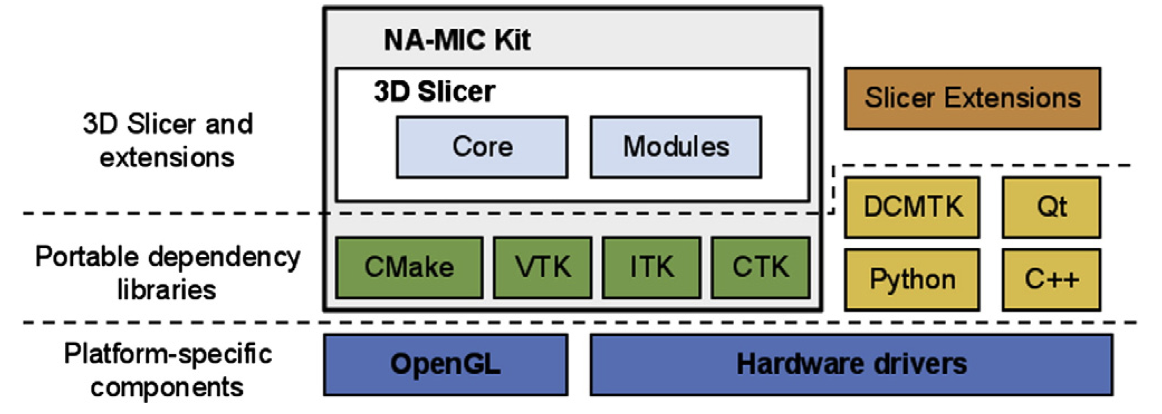
\includegraphics[width=1\textwidth]{img/3d_slicer_overview.jpg}
	\caption{3D Slicer Ökosystem nach \citet[S.~1326]{fedorov2012slicer}}
	\label{fig:3d_slicer_oekosystem}
\end{figure}

\citet[S.~1326]{fedorov2012slicer} teilt mit der Abbildung
\ref{fig:3d_slicer_oekosystem} die Plattform in drei Schichten auf. Auf der Obersten
wird klar, dass 3D Slicer aus der Kernanwendung und den installierbaren Modulen
besteht. Neben den bereits vorhandenen Modulen können, von externen Entwicklern
Module über die \textit{Slicer Extension} entwickelt und bereitgestellt werden.
Um eine Weiterentwicklung möglich zu machen hat Slicer eine Reihe von
Abhängigkeiten, die jedoch portabel gehalten werden. Auf der untersten Schicht
sind die Plattformspezifischen Anforderungen zu sehen, die Slicer erfüllen soll.
So kommt es, dass sich das 3D Slicer Ökosystem durch einige Kriterien auszeichnet,
die es besonders attraktiv für die Bearbeitung von medizinischen Bilddaten
machen. Zu den wichtigsten Vorteilen gehört die Tatsache, dass die Software
kostenfrei verfügbar ist. Darüber hinaus bietet sie eine umfassende Plug-in-Infrastruktur,
die über den sogenannten \textit{Extension-Manager} zugänglich ist. Dies
ermöglicht eine einfache Erweiterung der Funktionalitäten nach Bedarf. Ein weiteres
herausragendes Merkmal ist die Möglichkeit, Skripte direkt in der integrierten
Python-Konsole auszuführen. Schließlich ist 3D Slicer besonders für seine Vielseitigkeit
bekannt, da es medizinische Bilddaten aus sämtlichen Bereichen und in sämtlichen
Formaten der Medizin verarbeiten kann.

3D Slicer hat für alle diese Punkte jeweils eine Lösung entwickelt, wobei der erste
Punkt durch die Open-Source-Philosophie schon gegeben ist. Die folgenden
Abschnitte decken diese Lösungen ab und bilden so eine erste Grundlage für die
Entwicklung mit 3D Slicer.
% ---------------------------------------------------------------------------------------

\section{Plug-in-Infrastruktur}
Der wohl bedeutendste Punkt ist die Plug-in-Infrastruktur, welche Slicer von sich
aus mitbringt. Um dieses Konzept genauer zu beleuchten, teilt man die Plattform am
besten in zwei Teile auf, die Kernanwendung und die Module, welcher jeder Anwender
personalisiert installieren oder deinstallieren kann. Diese Module werden als
\textit{Slicer lodabel module} bezeichnet \citep[vgl.][S.~1332]{fedorov2012slicer}.
Slicer realisiert die Struktur durch den \textit{Extension Manager}, welcher durchaus
vergleichbar ist mit einer Art App-Store. Über diesen können bequem und mit
wenig Klicks die gewünschten Erweiterungen in das Kernsystem installiert werden.
Neben der Möglichkeit Module zu installieren bietet Slicer noch die Möglichkeit eigenen
Module zu bauen und Sie im \textit{Extension Manager} zu veröffentlichen. Diese werden
als \ac{SEM} bezeichnet. Abbildung \ref{fig:3d_slicer_extension_index} soll diesen
Vorgang verdeutlichen \citep[vgl.][]{slicer2024}.

\begin{figure}[h]
	\centering
	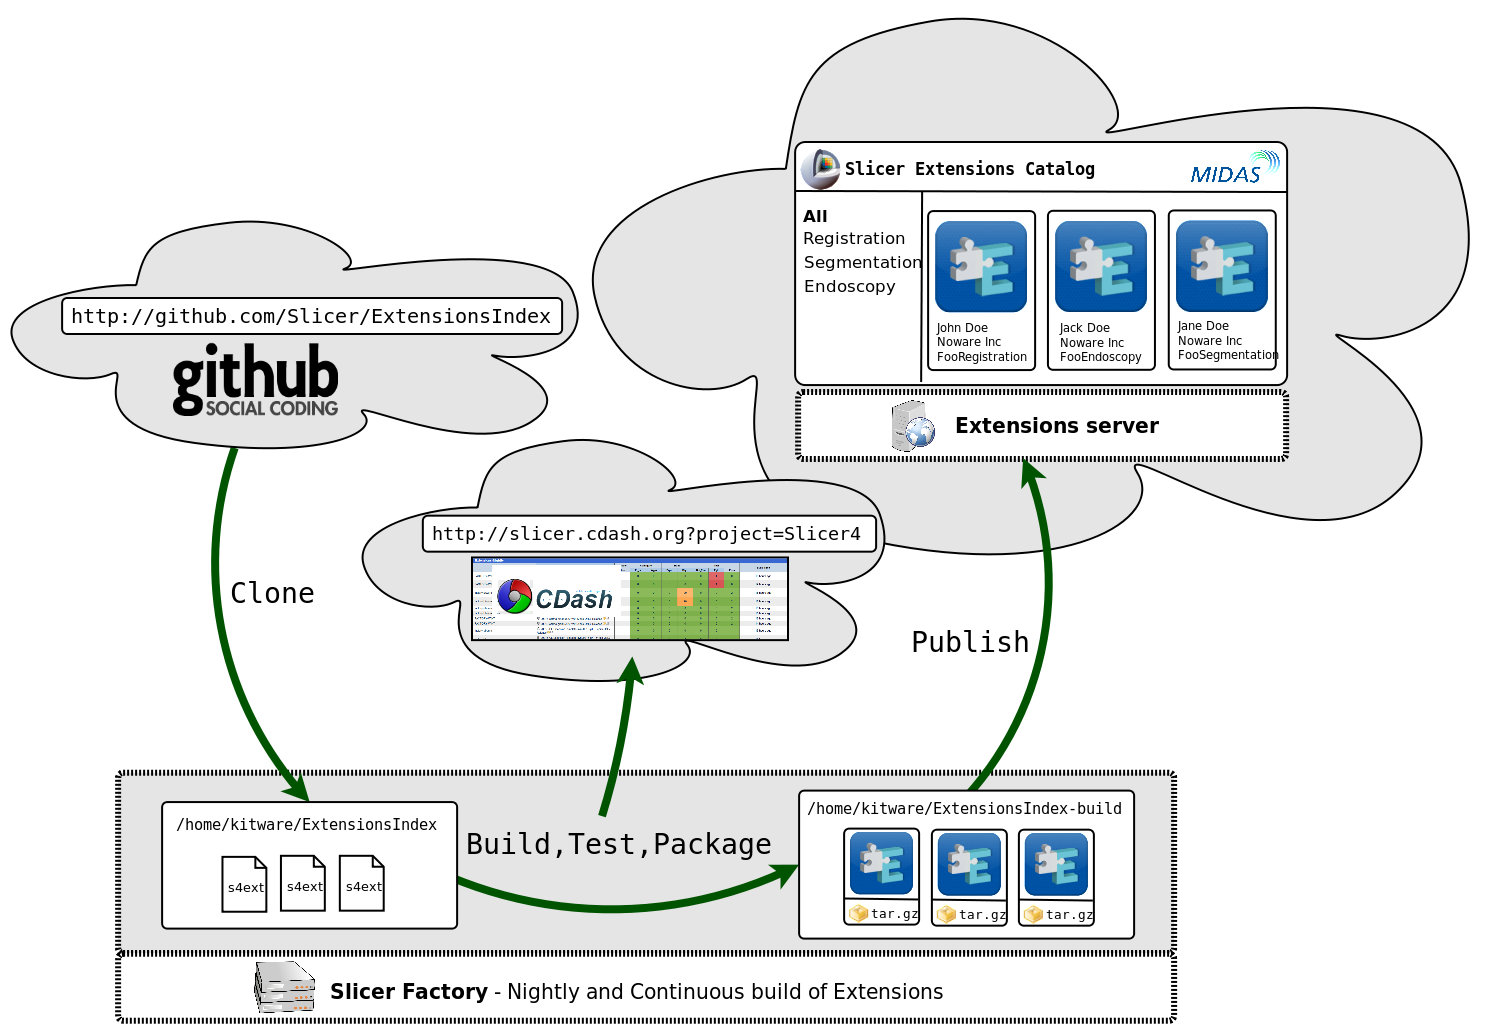
\includegraphics[width=0.5\textwidth]{img/slicer_extention_index.png}
	\caption{Funktionsweise der Plug-in-Infrastruktur von 3D Slicer nach \citet{extensionsIndex2024}}
	\label{fig:3d_slicer_extension_index}
\end{figure}

Slicer realisiert die Plug-in-Infrastruktur, indem die Plattform über ein
zusätzliches Repository verfügt, dass sich \href{https://github.com/Slicer/ExtensionsIndex?tab=readme-ov-file}{\textit{ExtensionIndex}}
nennt. Dieses öffentliche Repository ist eine Auflistung aller \ac{SEM}. Die
Auflistung erfolgt durch eine Reihe an \ac{JSON} Dateien, die auf den Quellcode
der einzelnen Erweiterungen verweisen. Dieser \href{https://github.com/Slicer/ExtensionsIndex?tab=readme-ov-file}{\textit{ExtensionIndex}}
ist über die Slicer Factory an den Extention Server und damit auch an den \textit{Extention
Manager} angebunden. Die Slicer Factory ist ein System, das aus einem Slicer
Extention Repository ein lauffähiges Build erstellt, welches in den Extention Katalog
eingebunden werden kann. Ist eine Erweiterung in dem Erweiterungskatalog
gelistet, so sorgt der \textit{Extension Manager} dafür, dass die von der Slicer
Factory erstellt Build-Datei installiert werden kann.

Während die Module von Slicer gebaut werden, werden parallel auch immer die
Tests für die Kernanwendung ausgeführt. Diese sind über ein Dashboard einsehbar.
So wird sichergestellt, dass keines der Module einen Fehler im Kernsystem verursacht.
Außerdem ist so für alle Benutzer von Slicer transparent einsehbar, in welchem Zustand
sich die Software gerade befindet. Die Kernanwendung von 3D Slicer folgt einem
Entwurfsmuster, dass sich \ac{MVC} nennt. Bei der Erstellung eines \ac{SEM} soll
dieser Ansatz ebenfalls gepflegt werden. Eine High Level Betrachtung der Softwarearchitektur
von 3D Slicer bietet \cite[S.~1332]{fedorov2012slicer} mit der Abbildung \ref{fig:3d_slicer_architektur}.

\begin{figure}[h]
	\centering
	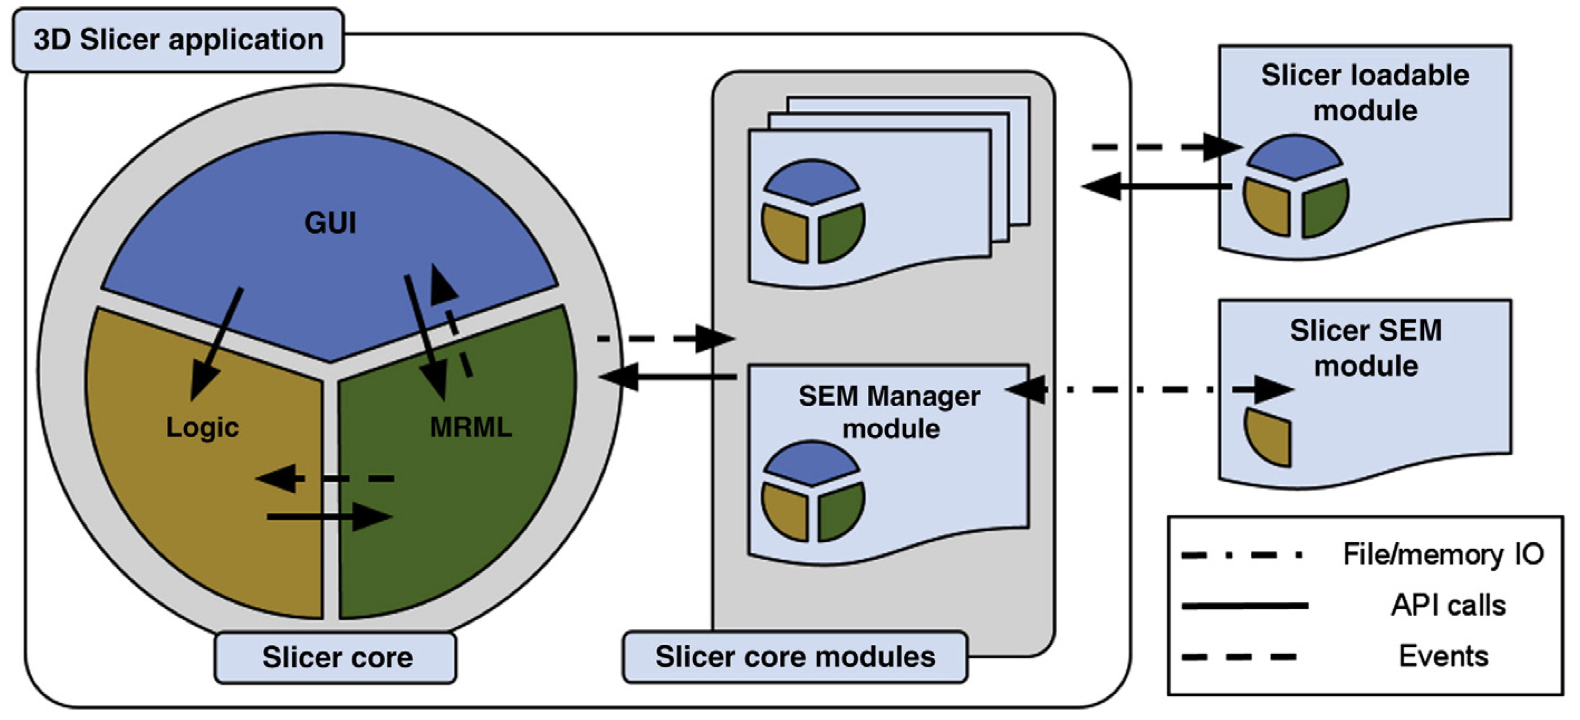
\includegraphics[width=0.7\textwidth]{img/3d_slicer_architektur.jpg}
	\caption{3D Slicer High Level Architektur nach \citet[S.~1332]{fedorov2012slicer}}
	\label{fig:3d_slicer_architektur}
\end{figure}

Das Zusammenspiel zwischen \ac{MRML}, \ac{GUI} und der Logik bilden das MVC-Pattern
in der Kernanwendung. Das identische Pattern spiegelt sich auch in den einzelnen
Modulen von Slicer wider. So wird sichergestellt, dass ein
Softwareentwicklungsparadigma eingehalten wird, was sich \textit{separation of
concerns} nennt. Die Kapselung von zusammengehöriger Logik. Bei der Erstellung
einer eigenen Erweiterung ist die Idee, dass nur die Logik implementiert werden muss
und die komplexe Architektur von Slicer erstmal nicht relevant ist.

Jedoch bietet sich in Slicer nicht nur die Möglichkeit eigene Erweiterungen zu erstellen,
es lässt sich hierfür auch die integrierte Python-Konsole nutzen.
% ---------------------------------------------------------------------------------------

\section{Python-Umgebung}
\label{subsec:pythob_umgebung} 3D Slicer bringt eine integrierte Python-Konsole
mit, über die mit der Datenstruktur interagiert werden kann. So ist es möglich, Python-Skripte
direkt in der Konsole auszuführen. Um dies zu realisieren, bringt Slicer mit der
Installation im jeweiligen Betriebssystem eine komplette Python-Umgebung mit.
Dieses sieht wie folgt aus.

\begin{center}
	\texttt{./Slicer/bin/PythonSlicer}
\end{center}

Diese Python-Umgebung verfügt über alle notwendigen Abhängigkeiten und Pakete.
Bei der Entwicklung eines \ac{SEM} kann dann auf die installierten Pakete in der
integrierten Python-Umgebung zurückgegriffen werden. So kommt es, dass für eine Entwicklung
mit Slicer keine eigene Python-Umgebung auf der lokalen Maschine installiert sein
muss. Slicer bringt hier alles mit. Für die Anwender, die eine terminal basierte
Bearbeitung vorziehen, besteht diese Möglichkeit nach wie vor.

Für den letzten charakteristischen Punkt von Slicer aus Kapitel \ref{sec:3d_slicer}
führt der nächste Abschnitt in die durchaus komplexe Datenstruktur \ac{MRML} ein,
die bei einer Entwicklung mit Slicer unausweichlich zu berücksichtigen ist.
% ---------------------------------------------------------------------------------------

\section{MRML-Datenstruktur}
\label{subsec:mrml_datenstruktur} Die \ac{MRML}, gesprochen \textit{"Murlm"} ist
ein Datenmodell, das dafür entwickelt wurde, alle möglichen Bilddaten zu
visualisieren und zu speichern, die für einen klinischen Zweck Einsatz finden \citep[vgl.][]{slicer2024}.
Laut \citet{slicer2024} wurde die \ac{MRML}-Datenstruktur völlig unabhängig von der
Slicer Kernanwendung entwickelt. Dies ermöglicht ein Portieren der Datenstruktur
auf andere Softwareapplikationen. Da Slicer die einzig große Plattform ist, die
diese Datenstruktur nutzt, wird der Quellcode für \ac{MRML} im Repository von 3D
Slicer gewartet und weiterentwickelt, so die \citet{slicer2024}. Durch den Artikel
von \citet[S.~1331]{fedorov2012slicer} wird klar, dass \ac{MRML} mehr ist also
nur eine Datenstruktur. Sie beschreiben \ac{MRML} als Szenenorganisator von
Bilder, Annotationen, Layouts und Anwendungsdaten. \citet[S.~1327]{fedorov2012slicer}
beschreiben die \ac{MRML}-Datenstruktur als Schlüsselkomponenten innerhalb von 3D
Slicer. Dies ist auf die Softwarearchitektur von Slicer zurückzuführen, die in Abbildung
\ref{fig:3d_slicer_architektur} beschrieben wurde. Die Kernanwendung von Slicer
arbeitet wie bereits beschrieben nach dem \ac{MVC}-Pattern. \ac{MRML} übernimmt hier
den Teil des \textit{Models (M)} und bildet damit den Grundstein der Anwendung
\citep[vgl.][S.~1332]{fedorov2012slicer}. \citet{slicer2024} beschreibt \ac{MRML}
als \ac{XML} Format. Wird also eine \ac{MRML}-Szene gespeichert, so folgt eine
Speicherung als \ac{MRML}-Datei und damit unter der Haube als \ac{XML}-Datei. Dabei
wird laut \citet{slicer2024} nur eine Referenz auf das Bild gespeichert. Die zu bearbeitende
Aufnahme selbst wird nicht innerhalb einer \ac{MRML}-Datei abgespeichert. \ac{MRML}
zeichnet sich vor allem dadurch aus, dass es eine Vielzahl an Dateiformaten akzeptiert.
Alle Formate, die für einen klinischen Zweck verarbeitet werden, können durch
\ac{MRML} unterstützt werden. Um dies zu gewährleisten, ist die \ac{MRML}-Szene
in sogenannte Knoten (engl.: nodes) aufgeteilt. Die Basistypen für einen Knoten folgen
der \citet{slicer2024} und sind in der folgenden Aufzählung zu sehen.

\begin{minipage}{0.45\textwidth}
	\begin{itemize}
		\item Data node

		\item Display node

		\item Storage node

		\item View node
	\end{itemize}
\end{minipage}
\hfill
\begin{minipage}{0.45\textwidth}
	\begin{itemize}
		\item Plot node

		\item Subject hierarchy node

		\item Sequence node

		\item Parameter node
	\end{itemize}
\end{minipage}

Wird also ein Bild in eine \ac{MRML}-Szene geladen, so speichert Slicer die unterschiedlichen
Eigenschaften eines Bildes in unterschiedlichen Knoten. So werden Beispielsweise
Basiseigenschaften einer Probe im \textit{Data node} gespeichert, wo hingegen
ein \textit{Storage node} beschreibt wie ein Bild auf der Festplatte gespeichert
wird. Im \textit{Display node} werden die Eigenschaften zur Darstellung eines Bildes
hinterlegt. Der Hintergrund für die Speicherung von Probendaten in
unterschiedlichen Knoten ist, dass beispielsweise dasselbe Bild in unterschiedlichen
Formaten vorliegt oder ein und dasselbe Bild auf zwei unterschiedliche Arten visualisiert
werden soll. So kann sich beispielsweise eine Struktur wie in Abbildung
\ref{fig:3d_slicer_class} ergeben.

\begin{figure}[h]
	\centering
	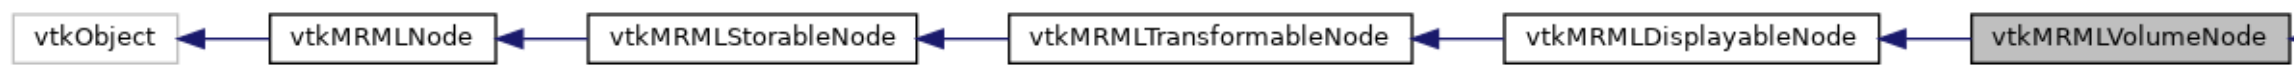
\includegraphics[width=1\textwidth]{img/slicer_class_index.jpg}
	\caption{Verkettung der einzelnen Knoten in der MRML-Datenstruktur nach \citet{slicer2024}}
	\label{fig:3d_slicer_class}
\end{figure}

Die Informationen in einem Bild werden also über diese Typen aufgeteilt und je nach
Sinn abgespeichert. Möchte man demnach auf die bestimmte Informationen in einer
Probe zugreifen, so kann diese Information über den Aufruf bestimmter Methoden erfolgen

\pagebreak

\begin{lstlisting}[
	language={python},
	caption={Auslesen der Informationen aus den verschiedenen Knoten},
	label={lst:_auslehsen_nodes}]
# data node - vtkMRMLVolumeNode
currentVolume.GetImageData()
# storage node - vtkMRMLStorableNode
currentVolume.GetStorageNode()
# display node - vtkMRMLDisplayableNode
currentVolume.GetDisplayNode()
\end{lstlisting}

Wie die Kommentare in Listing \ref{lst:_auslehsen_nodes} bereits zeigen, gibt es
noch eine Besonderheit von \ac{MRML}. Damit eine Verwaltung aller Dateiformate möglich
ist, bedient sich \ac{MRML} einiger Tools, die sich bereits etabliert haben. Die
Wichtigsten sind hierbei das \ac{VTK} und das \ac{ITK} \citep[vgl.][K.~1.1]{vtk2006},
\citep[vgl.][K.~1.1]{itkguide2015}. Die beiden Tools sind echte Riesen in ihrer Branche.
\ac{MRML} nutzt diese, um einige Dateiformate zu lesen und zu schreiben. Durch das
Betrachten der \ac{MRML}-Szene wird klar, dass Slicer hierdurch viele Möglichkeiten
bietet. Speziell für die effiziente Speicherung der Proben in einer Szene durch
die unterschiedlichen Knotentypen.

Mit dem Ende dieses Kapitels wurden alle wichtigen theoretischen Grundlage
besprochen, die notwendig sind um die anatomische Segmentierung über ein 3D Slicer
Modul bereitzustellen. Bevor die konkrete Methodik thematisiert wird, die für die
Entwicklung des Moduls angewendet wird, sollen im nächsten Kapitel kurz die
Rahmenbedingungen gesetzt werden, innerhalb deren entwickelt werden soll.
% ---------------------------------------------------------------------------------------